\scanpage{80}
\[
\underline{\underbrace{45.3}\,.\underbrace{32}\,.\underbrace{3}}:\unsure{\deleted{(3!3!)}|(3!3!)}=45.\deleted{\unsure{2|4}}.8\deleted{\unsure{2}}=2^3\,3^2\,5=360
\]
\[
\text{autom}\quad\underset{\substack{\Vert\\144}}{36.4}\ \big|\quad
(\unsure{\mathfrak S|\mathscr S}_3\times\mathfrak S_3).\mathfrak S_2\times\mathfrak S_2
\]
\figure{\begin{tikzpicture}[x=.032cm,y=-.032cm,line cap=round,line join=round]
\draw[gray!45] (1,37) -- (16,3) -- (46,39);


\end{tikzpicture}}
\figure{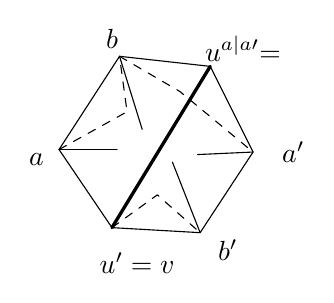
\begin{tikzpicture}[x=.032cm,y=-.032cm,line cap=round,line join=round]
\draw (7,40) -- (31,3) -- (67,7) -- (84,41) -- (63,73) -- (28,71) -- cycle;
\draw (7,40) -- (30,40);
\draw (62,42) -- (84,41);
\draw (31,3) -- (40,32);
\draw (52,45) -- (63,73);
\draw[very thick] (28,71) -- (67,7);
\draw[dashed] (7,40) -- (34,25) -- (31,3);
\draw[dashed] (28,71) -- (46,58) -- (63,73);
\draw[dashed] (31,3) -- (55,17) -- (84,41);
\node[inner sep=.5pt] at (-2,44) {$a$};
\node[inner sep=.5pt] at (28,-4) {$b$};
\node[inner sep=.5pt] at (80,0) {$u^{\unsure{a|a\prime}}{=}$};
\node[inner sep=.5pt] at (100,41) {$a'$};
\node[inner sep=.5pt] at (74,80) {$b'$};
\node[inner sep=.5pt] at (38,85) {$u'=v$};

\end{tikzpicture}}
\[
W_{\unsure{v|u}}(a).\quad w_u(b)\qquad
\underbrace{\unsure{\delta|J|\xi}_{12}\delta_{23}\delta_{34}}\ \underbrace{\delta_{45}\delta_{56}\delta_{64}}
\]
\[
w_v(a)-\{b\}\qquad\underline{\delta_i\delta'_{i'}}\quad 4\leq i\leq 6
\]
\figure{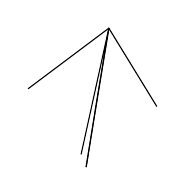
\begin{tikzpicture}[x=.032cm,y=-.032cm,line cap=round,line join=round]
\draw (0,24) -- (32,0) -- (51,31);
\draw (21,50) -- (32,0) -- (23,55);
\draw (23,55) -- (27,30) -- (32,0);


\end{tikzpicture}}
\figure{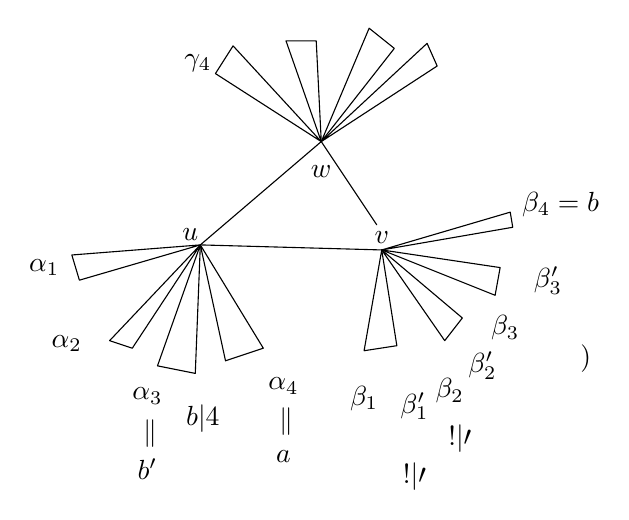
\begin{tikzpicture}[x=.032cm,y=-.032cm,line cap=round,line join=round]
\draw (45,81) -- (93,40) -- (115,73);
\draw (45,81) -- (117,83);
\draw (93,40) -- (51,13) -- (58,2) -- cycle;
\draw (93,40) -- (79,0) -- (91,0) -- cycle;
\draw (93,40) -- (112,-5) -- (122,3) -- cycle;
\draw (93,40) -- (135,1) -- (139,10) -- cycle;
\draw (45,81) -- (-3,95) -- (-6,85) -- cycle;
\draw (45,81) -- (9,119) -- (18,122) -- cycle;
\draw (45,81) -- (28,129) -- (43,132) -- cycle;
\draw (45,81) -- (55,127) -- (70,122) -- cycle;
\draw (117,83) -- (168,68) -- (169,74) -- cycle;
\draw (117,83) -- (164,90) -- (162,101) -- cycle;
\draw (117,83) -- (149,110) -- (142,119) -- cycle;
\draw (117,83) -- (123,121) -- (110,123) -- cycle;
\node[inner sep=.5pt] at (41,77) {$u$};
\node[inner sep=.5pt] at (117,78) {$v$};
\node[inner sep=.5pt] at (93,52) {$w$};
\node[inner sep=.5pt] at (44,9) {$\gamma_4$};
\node[inner sep=.5pt] at (-17,90) {$\alpha_1$};
\node[inner sep=.5pt] at (-8,120) {$\alpha_2$};
\node[inner sep=.5pt] at (24,141) {$\alpha_3$};
\node[inner sep=.5pt] at (25,156) {$\Vert$};
\node[inner sep=.5pt] at (24,170) {$b'$};
\node[inner sep=.5pt] at (46,150) {$\unsure{b|4}$};
\node[inner sep=.5pt] at (78,137) {$\alpha_4$};
\node[inner sep=.5pt] at (79,151) {$\Vert$};
\node[inner sep=.5pt] at (78,165) {$a$};
\node[inner sep=.5pt] at (188,65) {$\beta_4=b$};
\node[inner sep=.5pt] at (183,95) {$\beta'_3$};
\node[inner sep=.5pt] at (166,114) {$\beta_3$};
\node[inner sep=.5pt] at (157,129) {$\beta'_2$};
\node[inner sep=.5pt] at (144,139) {$\beta_2$};
\node[inner sep=.5pt] at (130,145) {$\beta'_1$};
\node[inner sep=.5pt] at (110,142) {$\beta_1$};
\node[inner sep=.5pt] at (148,158) {$\unsure{!|\prime}$};
\node[inner sep=.5pt] at (130,173) {$\unsure{!|\prime}$};
\node[inner sep=.5pt] at (198,126) {$)$};

\end{tikzpicture}}
\figure{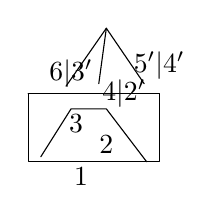
\begin{tikzpicture}[x=.032cm,y=-.032cm,line cap=round,line join=round]
\draw (2,27) -- (2,54) -- (54,54) -- (54,27);
\draw (2,27) -- (54,27);
\draw (7,52) -- (19,33) -- (33,33) -- (49,54);
\draw (17,24) -- (33,1) -- (48,23);
\draw (33,1) -- (30,23);
\node[inner sep=.5pt] at (23,60) {$1$};
\node[inner sep=.5pt] at (33,47) {$2$};
\node[inner sep=.5pt] at (21,39) {$3$};
\node[inner sep=.5pt] at (19,19) {$\unsure{6|3'}$};
\node[inner sep=.5pt] at (54,16) {$\unsure{5'|4'}$};
\node[inner sep=.5pt] at (40,27) {$\unsure{4|2'}$};

\end{tikzpicture}}
\unsure{Antiprisme|antiprisme|pentaprismes} $\sim$ couples de 3-bases voisines \deleted{et} bijection entre les deux --- couple d'une bibase et d'une partition de type $(3,3)$, avec iso. des deux morceaux i.e. isom. de $I$ (ens à 6 él) comme produit d'une de 3 par une de 2
\figure{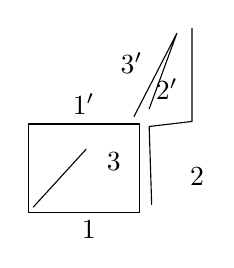
\begin{tikzpicture}[x=.032cm,y=-.032cm,line cap=round,line join=round]
\draw (0,38) -- (44,38) -- (44,73) -- (0,73) -- cycle;
\draw (2,71) -- (23,48);
\draw (49,70) -- (48,39) -- (65,37) -- (65,0);
\draw (42,35) -- (59,2) -- (48,32);
\node[inner sep=.5pt] at (24,80) {$1$};
\node[inner sep=.5pt] at (67,59) {$2$};
\node[inner sep=.5pt] at (34,53) {$3$};
\node[inner sep=.5pt] at (22,30) {$1'$};
\node[inner sep=.5pt] at (55,24) {$2'$};
\node[inner sep=.5pt] at (41,14) {$3'$};

\end{tikzpicture}}
\diagram{\begin{tikzcd}[ampersand replacement=\&,column sep=small,row sep=large]
a\arrow[r,dash]\arrow[d,dash] \& b\arrow[r,dash]\arrow[d,dash]\arrow[dl,dash] \& u\arrow[d,dash]\arrow[dl,dash]\\
a'\arrow[r,dash]\arrow[ur,dash,shift right] \& b'\arrow[r,dash] \& u'
\end{tikzcd}}
\par\noindent\rule{\linewidth}{.4pt}\par
\deleted{
\figure{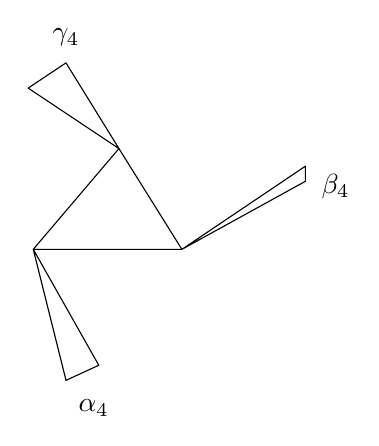
\begin{tikzpicture}[x=.032cm,y=-.032cm,line cap=round,line join=round]
\draw (7,74) -- (41,34) -- (66,74) -- cycle;
\draw (41,34) -- (5,10) -- (20,0) -- cycle;
\draw (66,74) -- (115,41) -- (115,47) -- cycle;
\draw (7,74) -- (20,126) -- (33,120) -- cycle;
\node[inner sep=.5pt] at (20,-10) {$\gamma_4$};
\node[inner sep=.5pt] at (127,49) {$\beta_4$};
\node[inner sep=.5pt] at (31,137) {$\alpha_4$};

\end{tikzpicture}}
\[
\begin{aligned}
U\mid P_u&=\mathrm{id} & V\unsure{\mid P_v)|(P_v)}&=\mathrm{id} & W(P_w)&=\mathrm{id}\\
U_{\deleted{\unsure{u|4}}}(\alpha_4)&=\alpha_4 & V\unsure{\mid(\beta_4)|(\beta_4)}&=\beta_4 & W(\gamma_4)&=\gamma_4
\end{aligned}
\]
\[
UVW\in\{1,\sigma\}\quad\overset{?}{\Longrightarrow}\quad U,V,W=1
\]
\diagram{\begin{tikzcd}[ampersand replacement=\&,row sep=small,column sep=small]
\&\unsure{K|\mathcal K|C}\arrow[r]\arrow[dl]\arrow[d]\arrow[dr]\& V\times V\times V\\
N_1\arrow[dr,equal] \& N_2\arrow[d,equal] \& N_3\arrow[dl,equal]\\
\&C\&
\end{tikzcd}}
\[
\begin{array}{cc}J&I\\\unsure{\wr\Vert|\Vert|\simeq}&\Vert\\V^*&\{u,v,w\}\end{array}
\]
\[
\underset{9}{I\times\{0,1,2\}}\ \amalg\
\underset{3}{I}\times\underset{3}{J}\times\underset{2}{\mathrm{Circ}(I)}
\]
}
% archive sheet number: 79
